
%%% Didn't love this class
%% Material isn't super deep (can't dive too much into the IO side)
%% Worried that the students already know the material

\documentclass[notes,11pt, aspectratio=169]{beamer}

\usepackage{pgfpages}
\usepackage{mdwlist}
% These slides also contain speaker notes. You can print just the slides,
% just the notes, or both, depending on the setting below. Comment out the want
% you want.
\setbeameroption{hide notes} % Only slide
%\setbeameroption{show only notes} % Only notes
%\setbeameroption{show notes on second screen=right} % Both

\usepackage{helvet}
\usepackage[default]{lato}
\usepackage{array}
\usepackage{tgbonum}
\usepackage[sfdefault]{FiraSans} %% option 'sfdefault' activates Fira Sans as the default text font
\usepackage[T1]{fontenc}
\renewcommand*\oldstylenums[1]{{\firaoldstyle #1}}

\usepackage{tikz}
\usepackage{verbatim}
\setbeamertemplate{note page}{\pagecolor{yellow!5}\insertnote}
\usetikzlibrary{positioning}
\usetikzlibrary{snakes}
\usetikzlibrary{calc}
\usetikzlibrary{arrows}
\usetikzlibrary{decorations.markings}
\usetikzlibrary{shapes.misc}
\usetikzlibrary{matrix,shapes,arrows,fit,tikzmark}
\usepackage{amsmath}
\usepackage{mathpazo}
\usepackage{hyperref}
\usepackage{lipsum}
\usepackage{multimedia}
\usepackage{graphicx}
\usepackage{multirow}
\usepackage{graphicx}
\usepackage{dcolumn}
\usepackage{bbm}
\newcolumntype{d}[0]{D{.}{.}{5}}

\usepackage{changepage}
\usepackage{appendixnumberbeamer}
\newcommand{\beginbackup}{
   \newcounter{framenumbervorappendix}
   \setcounter{framenumbervorappendix}{\value{framenumber}}
   \setbeamertemplate{footline}
   {
     \leavevmode%
     \hline
     box{%
       \begin{beamercolorbox}[wd=\paperwidth,ht=2.25ex,dp=1ex,right]{footlinecolor}%
%         \insertframenumber  \hspace*{2ex} 
       \end{beamercolorbox}}%
     \vskip0pt%
   }
 }
\newcommand{\backupend}{
   \addtocounter{framenumbervorappendix}{-\value{framenumber}}
   \addtocounter{framenumber}{\value{framenumbervorappendix}} 
}


\usepackage{graphicx}
\usepackage[space]{grffile}
\usepackage{booktabs}
\newcommand\independent{\protect\mathpalette{\protect\independenT}{\perp}}
\def\independenT#1#2{\mathrel{\rlap{$#1#2$}\mkern2mu{#1#2}}}
\DeclareMathOperator{\Supp}{Supp}

% These are my colors -- there are many like them, but these ones are mine.
\definecolor{blue}{RGB}{0,114,178}
\definecolor{red}{RGB}{213,94,0}
\definecolor{yellow}{RGB}{240,228,66}
\definecolor{green}{RGB}{0,158,115}

\hypersetup{
  colorlinks=false,
  linkbordercolor = {white},
  linkcolor = {blue}
}


%% I use a beige off white for my background
\definecolor{MyBackground}{RGB}{255,253,218}

%% Uncomment this if you want to change the background color to something else
%\setbeamercolor{background canvas}{bg=MyBackground}

%% Change the bg color to adjust your transition slide background color!
\newenvironment{transitionframe}{
  \setbeamercolor{background canvas}{bg=yellow}
  \begin{frame}}{
    \end{frame}
}

\setbeamercolor{frametitle}{fg=blue}
\setbeamercolor{title}{fg=black}
\setbeamertemplate{footline}[frame number]
\setbeamertemplate{navigation symbols}{} 
\setbeamertemplate{itemize items}{-}
\setbeamercolor{itemize item}{fg=blue}
\setbeamercolor{itemize subitem}{fg=blue}
\setbeamercolor{enumerate item}{fg=blue}
\setbeamercolor{enumerate subitem}{fg=blue}
\setbeamercolor{button}{bg=MyBackground,fg=blue,}



% If you like road maps, rather than having clutter at the top, have a roadmap show up at the end of each section 
% (and after your introduction)
% Uncomment this is if you want the roadmap!
% \AtBeginSection[]
% {
%    \begin{frame}
%        \frametitle{Roadmap of Talk}
%        \tableofcontents[currentsection]
%    \end{frame}
% }
\setbeamercolor{section in toc}{fg=blue}
\setbeamercolor{subsection in toc}{fg=red}
\setbeamersize{text margin left=1em,text margin right=1em} 

\newenvironment{wideitemize}{\itemize\addtolength{\itemsep}{10pt}}{\enditemize}

\usepackage{environ}
\NewEnviron{videoframe}[1]{
  \begin{frame}
    \vspace{-8pt}
    \begin{columns}[onlytextwidth, T] % align columns
      \begin{column}{.70\textwidth}
        \begin{minipage}[t][\textheight][t]
          {\dimexpr\textwidth}
          \vspace{8pt}
          \hspace{4pt} {\Large \sc \textcolor{blue}{#1}}
          \vspace{8pt}
          
          \BODY
        \end{minipage}
      \end{column}%
      \hfill%
      \begin{column}{.38\textwidth}
        \colorbox{green!20}{\begin{minipage}[t][1.2\textheight][t]
            {\dimexpr\textwidth}
            Face goes here
          \end{minipage}}
      \end{column}%
    \end{columns}
  \end{frame}
}

\title[]{\textcolor{blue}{Likelihood Methods II: Multiple Discrete Choices}}
\author[PGP]{}
\institute[FRBNY]{\small{Paul Goldsmith-Pinkham}}
\date{\today}


\begin{document}

%%% TIKZ STUFF
\tikzset{   
        every picture/.style={remember picture,baseline},
        every node/.style={anchor=base,align=center,outer sep=1.5pt},
        every path/.style={thick},
        }
\newcommand\marktopleft[1]{%
    \tikz[overlay,remember picture] 
        \node (marker-#1-a) at (-.3em,.3em) {};%
}
\newcommand\markbottomright[2]{%
    \tikz[overlay,remember picture] 
        \node (marker-#1-b) at (0em,0em) {};%
}
\tikzstyle{every picture}+=[remember picture] 
\tikzstyle{mybox} =[draw=black, very thick, rectangle, inner sep=10pt, inner ysep=20pt]
\tikzstyle{fancytitle} =[draw=black,fill=red, text=white]
%%%% END TIKZ STUFF

% Title Slide
\begin{frame}
\maketitle

\end{frame}


\begin{frame}{Today's topic: multiple discrete choice}
  \begin{columns}[T] % align columns
    \begin{column}{.7\textwidth}
      \begin{wideitemize}
      \item We'll now examine multiple discrete choice problems 
      \item Much of this discussion is very IO-adjacent
        \begin{itemize}
        \item However, many of these ideas are important for
          non-IO problems, e.g. multiple IVs and Roy models
        \item Moreover, these tools are very promising in fields that
          have not yet used them
        \end{itemize}
      \item Issues with choice problems that we'll discuss:
        \begin{itemize}
        \item Independence of Irrelevant Alternatives (IIA)
        \item Choice sets and consideration sets
        \item Inconsistency of fixed effects and its consequences
        \end{itemize}
      \end{wideitemize}
    \end{column}%
  \hfill%
  \begin{column}{.4\textwidth}
  \end{column}
\end{columns}
\end{frame}


\begin{frame}{Thinking about multiple choices}
  \begin{wideitemize}
  \item   Consider the following problem: we observe choices for individuals
    $Y_{i} = j$, $j \in \Omega = \{0, 1, \ldots, J\}$, where
    $J+1 = |\Omega|$ is the total number of choices.
    \begin{itemize}
    \item Importantly, the order of the choices has no particular
      meaning. This could be red bus, blue bus and car as
      transportation choices.
    \end{itemize}
  \item We observe three types of characteristics:
    \begin{enumerate}
    \item $X_{i}$ (individual chaaracteristics, invariant to choices),
    \item       $X_{j}$ (choice characteristics) 
    \item  $X_{ij}$ includes individual-by-choice characteristics
    \end{enumerate}
  \item Can write $X_{i}$ as $X_{ij}$ by interacting with choice
      fixed effects
    \begin{itemize}
  \item Note that when $J = 1$, we collapse down to binary choice
    \end{itemize}
  \end{wideitemize}
\end{frame}


\begin{frame}{Modeling multiple choices}
    \begin{wideitemize}
    \item Recall from last class that there are two ways to think
      about how we think about the discrete choice problem. These are not
      mutually exclusive.
    \item The first is a statistical view. How do we model the
      classification of a particular choice.
      \begin{itemize}
      \item In the binary choice problem, there is only one parameter
        that needs be known, conditional on $X_{i}$: 
        $\pi(X_{i}) = Pr(Y_{i} = 1 |X _{i})$
      \item With more than two choices, the dimensionality becomes
        more complicated.  We now have
        $\pi_{j}(\mathbf{X}), j=2,3$ for 3 choices. 
      \end{itemize}
    \item How should we parameterize how other choices' characteristics
      affect each other?
    \item Most of the models we will discuss today will make very
      specific restrictions on how choices affect one another
      \begin{itemize}
      \item These are not innocuous choices, as we'll see.
      \end{itemize}
  \end{wideitemize}
\end{frame}


\begin{frame}{The naive approach}
  \begin{wideitemize}
  \item If we want to estimate simple treatment effects, we could
    focus on binary outcomes
  \item For exmaple: we have a randomly assigned treatment $T$, and
    $J$ choices. What is the effect of $T$ on $Pr(Y_{i} = j)$?
  \begin{itemize}
  \item    $\tau_{j} = Pr(Y_{i} = j | T_{i} = 1) -Pr(Y_{i} = j | T_{i} = 0)$
  \end{itemize}
\item   There's less information about the substitution
  patterns of individuals in this form
\item Of course, it is still very helpful! And useful when faced with
  a lot of choices to focus on the effect on one margin.
\item However, need more structure to estimate relative choice
  substitution across outcomes
  \begin{itemize}
  \item E.g. what is the effect of $T$ on choosing $j$ conditional on
    choosing $j$ or $k$
  \end{itemize}
  \end{wideitemize}
\end{frame}

\begin{frame}{What's the estimand/counterfactual? }
  \begin{wideitemize}
  \item What counterfactual question are we interested in?
    \begin{enumerate}
  \item How does changing $X_{ij}$ affect the probability
    of choosing choice $j$ relative to all other choices?
  \item How does changing $X_{ij}$ affect the probability
    of choosing choice $j$ \emph{relative} to choice $k$?
  \item How does adding or subtracting one of the choices (with
    difference in $X_{ij}$) change the $J+1$ choice probabilities?
  \end{enumerate}
\item An important question is under what settings are these questions
  identified. In the examples we'll look at, there are answers that
  fall out (at least for 1 and 2) but they may be too driven by the
  parametric assumptions.
  \begin{itemize}
  \item See Berry and Haile (2016) for a discussion of identification
    in product markets in non-parametric settings.
  \item They show that there are two specific conditions that need to
    hold in the structure of the problem, but allow for very general
    structure in the distribution of the shocks.
  \end{itemize}
  \end{wideitemize}
\end{frame}

\begin{frame}{Modeling multiple choices}
    \begin{wideitemize}
    \item A second way to view this is as an structural (economic)
      choice problem (pioneered by McFadden). Consider a set of
      utilities $U_{ij}$ (unobserved) such that the
      $$Y_{i} = \arg\max_{j \in \Omega}U_{ij}$$
    \item E.g., person $i$ chooses $j$ if it's the choice that
      maximizes the utility amongst all $J+1$ choices.
      \begin{itemize}
      \item Note the similarity to the $Y^{*}_{i}$ in the binary case
      \end{itemize}

    \item If we make the assumptions:
      \begin{enumerate}
      \item  $U_{ij} = X_{ij}'\beta + \epsilon_{ij}$
      \item $\epsilon_{ij}$ are independent across choices and
        individuals, and distributed Type-I extreme value
      \end{enumerate}
      then we get the McFadden conditional logit model:
      $$Pr(Y_{i} = j | X_{ij}) = \frac{\exp(X_{ij}\beta)}{\sum_{k}\exp(X_{ik}\beta)}.$$
  \end{wideitemize}
\end{frame}

\begin{frame}{The impact of price}
  \begin{wideitemize}
  \item In many choice problems, a key parameter we're interested in
    is a price elasticity
  \begin{itemize}
  \item A key variable in $X_{ij}$ is $p_{j}$
  \item This term can be something else, but price matters quite a bit in IO
  \end{itemize}
  $$Pr(Y_{i} = j | X_{ij}) = \frac{\exp(p_{j}\gamma + X_{ij}\beta)}{\sum_{k}\exp(p_{k}\gamma +  X_{ik}\beta)}.$$
\item Own price elasticity is easily constructed from this:
      $$\epsilon_{j} = \frac{\partial Pr(Y_{i} = j | X_{ij})}{\partial p_{j}}\frac{p_{j}}{Pr(Y_{i} = j | X_{ij})}.$$
    \item This is not much different than calculating an average
      effect. What is more meaningful is that we can think about
      \emph{cross}-elasticities:
      $$\epsilon_{jk} = \frac{\partial Pr(Y_{i} = j | X_{ij})}{\partial p_{k}}\frac{p_{k}}{Pr(Y_{i} = j | X_{ij})}$$
    \end{wideitemize}
\end{frame}

\begin{frame}{Independence of Irrelevant Alternatives (IIA)}
  \begin{wideitemize}
  \item A key issue with this formulation of the conditional logit
    model -- the cross-elasticities are identical
    \begin{itemize}
    \item In other words, $\epsilon_{jk} = \epsilon_{lk}$
    \item The effect of shifting price of a different good causes an
      identical proportionate shift in all choices' market share
    \end{itemize}
  \item   Solve:
    \begin{align*}
      \epsilon_{jk} &= \underbrace{-\gamma Pr(Y_{i} = j )Pr(Y_{i} = k )}_{\frac{\partial Pr(Y_{i} = j)}{\partial p_{k}}} \times \frac{p_{k}}{Pr(Y_{i} = j | X_{ij})}\\
                    &= -\gamma Pr(Y_{i} = k )p_{k}
    \end{align*}
    \item Note that this is not a function of $j$, and hence identical for
    all other products
  \end{wideitemize}
  
\end{frame}

\begin{frame}{Independence of Irrelevant Alternatives (IIA)}
  \begin{wideitemize}
  \item Another way to see this problem: consider the probability of
    choosing $j$, conditional on choosing just $j$ and $k$:
    $$Pr(Y_{i} = j | Y_{i} \in \{j,k\}) = \frac{\exp{(X_{ij}\beta})}{\exp{(X_{ij}\beta)} + \exp{(X_{ik}\beta})} $$
  \item Note that none of the other choices show up in this
    probability choice -- irrespective of how ``similar'' the other
    choices are to $j$ or $k$.
    \begin{itemize}
    \item In other words, if a characteristic of the other products changes,
      the relative share between $j$ and $k$ will stay same
    \end{itemize}
  \item The canonical example of this is the ``car, red bus and
    blue bus'' example.
    \begin{itemize}
    \item  Presumably a person is purely indifferent
      between red and blue busses.
    \item Hence, a shift in the red bus price would cause a bigger substitution from the blue bus than from car
      users.
    \item Conditional logit (in this form) will not account for this
    \end{itemize}
  \end{wideitemize}
\end{frame}


\begin{frame}{How can we deal with this?}
  \begin{wideitemize}
    \item Better substitution patterns

    \item Note that this is an economics problem -- e.g. we have
      economic intuition about the market substitution patterns, and
      we don't think identical cross-elasticities makes sense
    
    \item It's also a statistical problem -- there is a very strong
    statistical functional form we have assummed, which was
    analytically convenient but has somewhat perverse properties

    \item Will talk about two ways to solve this (there are more in the IO literature):
    \begin{enumerate}
    \item Nested Logit and Correlated Multivariate Probit
    \item Random Coefficients Logit
    \end{enumerate}
  \end{wideitemize}
\end{frame}

\begin{frame}{Nested Logit and Correlated Multivariate Probit}
  \begin{wideitemize}
  \item One part of the problem comes from the independence of the
    $\epsilon$ across choices
    \begin{itemize}
    \item Recall that these $\epsilon$ effectively rationalize seeing
      non-zero choices in both directions, conditional on charcteristics
    \end{itemize}
  \item Recall the blue and red bus case:
    \begin{itemize}
    \item Getting two independent $\epsilon$ draws for the busses is not an intuitive
      view of bus demand
    \item Instead, the blue and bus likely have highly
      correlated epsilon draws (if not identical)
    \item The issue, of course, is what the correlation is within sets 
    \end{itemize}
  \item With the nested Logit approach, you can specify sets (as the
    researcher), and allow data-driven measures of correlation of the
    $\epsilon$ within these sets.
  \item The key is that the errors are uncorrelated across choice sets, which preserves
    the simple logit structure (see Goldberg (1995) for an example application)
  \end{wideitemize}
\end{frame}

\begin{frame}{Multivarite Probit}
    \begin{wideitemize}
    \item A more general approach is to allow the covariance matrix of
      the error terms to be flexibly estimated by the data using a multivariate normal
      \begin{itemize}
      \item E.g. $\epsilon_{i} = (\epsilon_{i0},\epsilon_{i1},\ldots, \epsilon_{iJ}) \sim \mathcal{N}(0, \Sigma)$
      \item Directly estimate $\Sigma$
      \end{itemize}
    \item This problem gets hard with many choices (parameter space grows at rate $J^{2}$)
    \item Importantly, do need to normalize one of the variance terms,
      since the variance matrix is only identified up to scale of one
      of the terms.
    \item See McCulloch, Pelson and Rossi (2000) for details in the
      Bayesian setting, and Train (2009) for simulation discussions in
      the frequentist case
      \begin{itemize}
      \item See Hull (2020) for a nice application
      \end{itemize}
  \end{wideitemize}
\end{frame}


\begin{frame}{Better substitution patterns - Random Coefficients}
  \begin{wideitemize}
  \item Rather than directly target the distribution of the
    $\epsilon_{ij}$, an alternative approach is to add more richness
    to the coefficients themselves
    \begin{itemize}
    \item By adding more random variation in this, it effectively
      creates a richer substitution pattern
    \end{itemize}
  \item Now consider a slight extension of our previous model, with
    $\beta_{i}$ varying by individual (in an unobserved way):
    \begin{align*}
      U_{ij} &= X_{ij}\beta_{i} + \epsilon_{ij}\\
      U_{ij} &= X_{ij}\overline{\beta} + \nu_{ij}, \qquad \nu_{ij} = \epsilon_{ij} + X_{ij}(\beta_{i}-\overline{\beta})
    \end{align*}
  \item There are a number of ways to estimate this approach, but
    notice the key point -- subtitution patterns are more richly
    modeled (and allowed) due to $\nu_{ij}$ varying by $X_{ij}$
    \begin{itemize}
    \item See McFadden and Train (2000) for details
    \end{itemize}
  \end{wideitemize}
\end{frame}

\begin{frame}{Symmetric unobserved product differentiation}
  \begin{wideitemize}
  \item The unobservable $\epsilon$ is an unobserved valuation of some
    product characteristic
    \begin{itemize}
    \item Most models (including the ones we've looked at) have
      symmetric unobserved product differentiation (SUPD) [Ackerberg and Rysman (2005)]
    \end{itemize}
  \item Consider our bus and car example -- the issue is that adding
    another bus product in this space should ``crowd'' the original bus market share
    \begin{itemize}
    \item E.g. the choices are highly correlated
    \end{itemize}
  \item This is beyond just IIA's effect of cross-price elasticities
    -- this matters when considering counterfactuals where you add new
    choices
    \begin{itemize}
    \item Let $X_{i}$ define the \emph{characteristic space}
    \item If a new product is added in the
      characteristic space, we think that they should crowd one
      another. With logit errors, they do not
    \end{itemize}
  \item Ackerberg and Rysman (2005) propose a solution that
    incorporates the number of choices directly
  \item The symmetry of our errors also plays an important role in
    making the cross price elasticities identical --
    e.g. $\epsilon_{ij} = \epsilon_{ji}$
  \end{wideitemize}
\end{frame}

\begin{frame}{Choice sets and consideration sets}
  \begin{wideitemize}
  \item In these discussions, we've assumed that all individual use the same choices
  \item Reasons why this could not be true are many: attention,
    knowledge, opportunity
    \begin{itemize}
    \item Call the subset of choices a consumer focuses on the
      \emph{consideration} set
    \item These can be known (observed) or usually, unknown
    \end{itemize}
  \item If we assert consideration sets are the full choice set for
    all individuals, when we see individuals choose certain goods, we
    view this as reflecting their preferences
    \begin{itemize}
    \item Or in other words, the counterfactual we generate from this
      model would imply a certain response
    \item E.g. if I never considered going to Harvard in my choice
      set, a change in its price will be irrelevant for me
    \end{itemize}
  \item If changes in characteristics affect your consideration set,
    this can have important implications for counterfactuals
  \end{wideitemize}
\end{frame}

\begin{frame}{Choice sets and consideration sets}
  \begin{wideitemize}
  \item The general way to view consideration sets in choice problems
    is
  \begin{equation*}
    s_{j}(p) = \sum_{C \in P(j)} \pi_{C}(p) s_{j}^{*}(p | C),
  \end{equation*}
  where
  \begin{itemize}
  \item $P(j)$ is the set of consideration sets that include choice $j$,
  \item  $s_{j}$ is the overall choice set of $j$ given prices $p$,
  \item  $\pi_{C}$ is the probability of consideration set $C$
  \item   $s_{j}^{*}$ is the choice of $j$ within the choice $C$ 
  \end{itemize}
\item Note that the key feature of this model is that it can break the
  symmetry of choice elasticities
  \begin{itemize}
  \item There is symmetry \emph{within} the consideration set
  \end{itemize}
\item Under certain modeling assumptions, it is possible to identify
  the probabilities of the consideration set choice (Abaluck and
  Adams-Prassl (2020))
\end{wideitemize}
\end{frame}

\begin{frame}{Bias from ignoring consideration sets}
  \begin{center}
  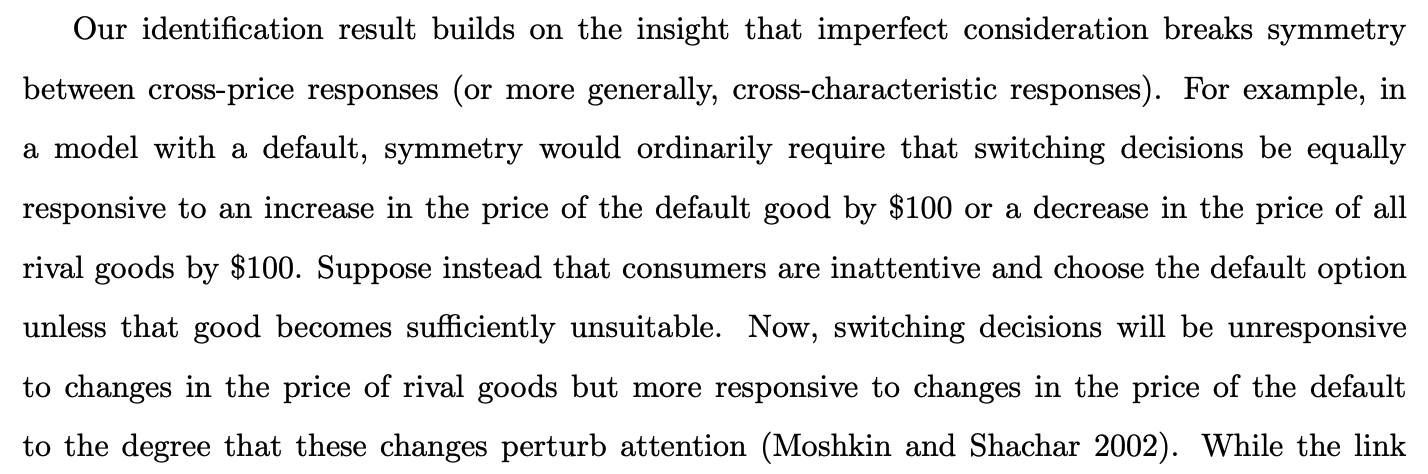
\includegraphics[width=\linewidth]{images/abaluck1.png}\\
  ...
  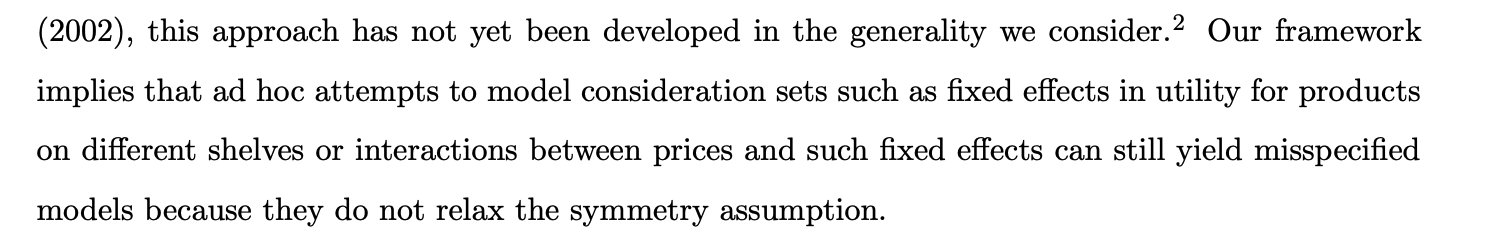
\includegraphics[width=\linewidth]{images/abaluck2.png}  
\end{center}
\end{frame}
\begin{frame}{Choice sets and consideration sets}
  \begin{wideitemize}
  \item Simple case considered in paper is when there is a base
    default that people focus on (and ignore other choices)
    \begin{itemize}
    \item Default Specific Model
    \end{itemize}
  \item More rich setting: Alternative Specific Choice model
    \begin{itemize}
    \item Put structure on how a choice is selected into a consideration set
    \end{itemize}
  \item In both cases, can identify the consideration choice
    probabilities using price elasticities
  \item This can be a very important thing to model if your
    counterfactual relates to changes in the consideration set
    \begin{itemize}
    \item However, it may not be first order to your problem at hand
    \end{itemize}
  \end{wideitemize}
\end{frame}

%%% UPDATE
\begin{frame}{BLP}
  \begin{wideitemize}
  \item Another important set of models is known as BLP (Berry
    Levinsohn Pakes)
    $$ U_{ijm} = \mu_{ijm} + \delta_{jm} + \epsilon_{ijm}$$
  \item This exploits knowledge of choices (either aggregated or
    disaggreated) across many markets
  \item Can use this knowledge to allow for a lot more market-product
    specific fixed effects ($\xi_{jm}$), which gives a richer
    substitution pattern
  \item Under distributional assumptions for $\epsilon_{ijm}$,
    \begin{equation}
      s_{jm}(\boldsymbol{\delta}_{m}, \beta) = \int \frac{\exp(\delta_{jm} + \mu_{ijm})}{\sum_{k \in J_{m}} \exp(\delta_{km} + \mu_{ikm})} f(\boldsymbol{\mu}|\beta) d \boldsymbol{\mu}_{im}
    \end{equation}
  \end{wideitemize}
\end{frame}

\begin{frame}{BLP}
    \begin{align*}
      s_{jm}(\boldsymbol{\delta}_{m}, \beta) &= \int \frac{\exp(\delta_{jm} + \mu_{ijm})}{\sum_{k \in J_{m}} \exp(\delta_{km} + \mu_{ikm})} f(\boldsymbol{\mu}|\beta) d \boldsymbol{\mu}_{im}\\
      \delta_{jm} &= x_{jm}\beta_{2} - \alpha p_{jt} + \xi_{jm}
    \end{align*}
  \begin{wideitemize}
  \item Key insight in BLP is to use a fixed point algorithm to match the estimated market shares in a market, $\hat{s}_{m}(\boldsymbol{\delta}_{m}, \beta)$, to the observed market shares
    \begin{itemize}
    \item This is done iteratively, mapping the shares into a linear index for $\delta$
    \item Conlon and Gortmaker (2020) highlight that this can have
      estimation issues due to convergence in this process
    \item Provide Python package to solve this!
    \end{itemize}
  \end{wideitemize}
\end{frame}


\begin{frame}{Inconsistency in binary choice models}
  \begin{wideitemize}
  \item One issue that arises in many non-linear binary choice model is that many
    features do not carry over from linear models
    \begin{itemize}
    \item E.g. interpreting coefficients is more challenging
    \item A bigger issue comes from  inconsistency of fixed effects
    \end{itemize}
\vspace{-5pt}    
  \item Consider estimating a panel fixed effects model with binary choice:
    \begin{align*}
      Y_{it} &= \alpha_{i} + X_{it}\beta + \epsilon_{it}\\
      Y_{it} &= F(\alpha_{i} + X_{it}\beta)
    \end{align*}
    where we are interested in the parameter $\beta$. If we have a
    short panel (e.g. few time periods), we cannot consistently
    estimate $\alpha_{i}$. However, in the linear case, this does not
    affect estimation of $\beta$
  \item Unique result (Chamberlain (1987,2010)): for binary
    outcome case, the only model that
    consistently estimates $\beta$ is a conditional logit
  \item More generally if you have inconsistent fixed effects in your
    non-linear models, this can cause serious issues (except in
    special cases like this one)
    \begin{itemize}
    \item OLS is good!
    \end{itemize}
  \end{wideitemize}
\end{frame}

\begin{frame}{Underlying structure of discrete choice is valuable in IV settings}
  \begin{wideitemize}
  \item Much of this discussion centered on IO style applications
  \item But this discussion shows up when thinking about Roy style models
  \item When we discuss instruments and individuals' choice to take up
    a policy or not, if the policy is multi-dimensional, this types of
    models play a huge role
  \item Recall our discussion of propensity scores for treatment effects
    \begin{itemize}
    \item If individuals choose between multiple treatment options,
      this maps directly into a discrete choice setting like what
      we've discussed today
    \end{itemize}
  \item Thinking carefully about the counterfactual pattern across
    will give guidance in more complicated IV settings
  \end{wideitemize}
  
\end{frame}

\begin{frame}{Arbitraging IO methods in other settings}
  \begin{wideitemize}
  \item Many fields have discrete choice applications but have not
    adopted the tools
  \item The cutting edge of IO tools is quite complex, but this type of
    structure is very valuable when thinking about complicated choice patterns
  \item Worthwhile to try to arbitrage these methods in fields that
    are less exposed to them (e.g. Koijen and Yogo (2019))
  \end{wideitemize}
\end{frame}

%%% UPDATE WITH KOIJEN AND YOGO

\begin{frame}{Koijen and Yogo (2019)}
  \begin{columns}[T] % align columns
    \begin{column}{.5\textwidth}
      \begin{wideitemize}
      \item Influential paper by Koijen and Yogo (2019) estimates a
        demand system for financial assets
      \item The framework is used to study three things:
        \begin{enumerate}
        \item Distribution of price elasticities with respect to demand shocks (residual demand)
        \item Decomposing variation in asset returns
        \end{enumerate}
      \end{wideitemize}
    \end{column}%
  \hfill%
  \begin{column}{.5\textwidth}
    \only<1>{  
\includegraphics[width=\linewidth]{images/koijenyogo.pdf}}
    \only<2>{  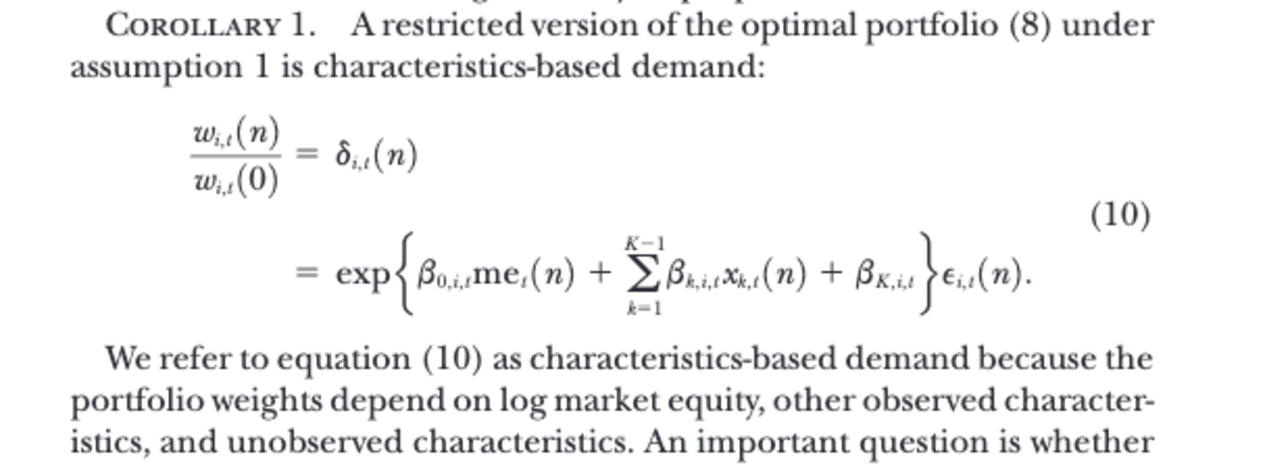
\includegraphics[width=\linewidth]{images/koijenyogo4.pdf}}
    \only<3>{  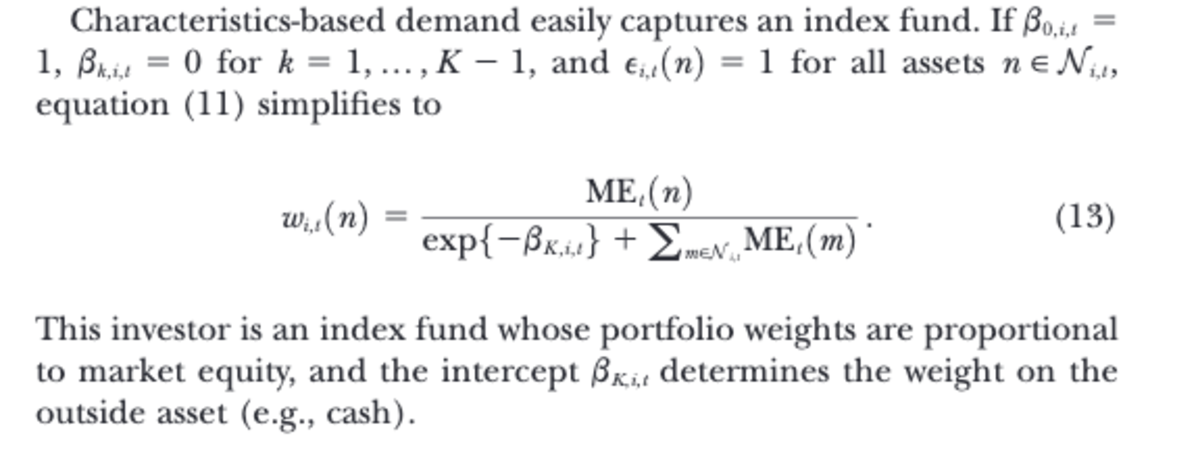
\includegraphics[width=\linewidth]{images/koijenyogo3.pdf}}
    \only<4>{  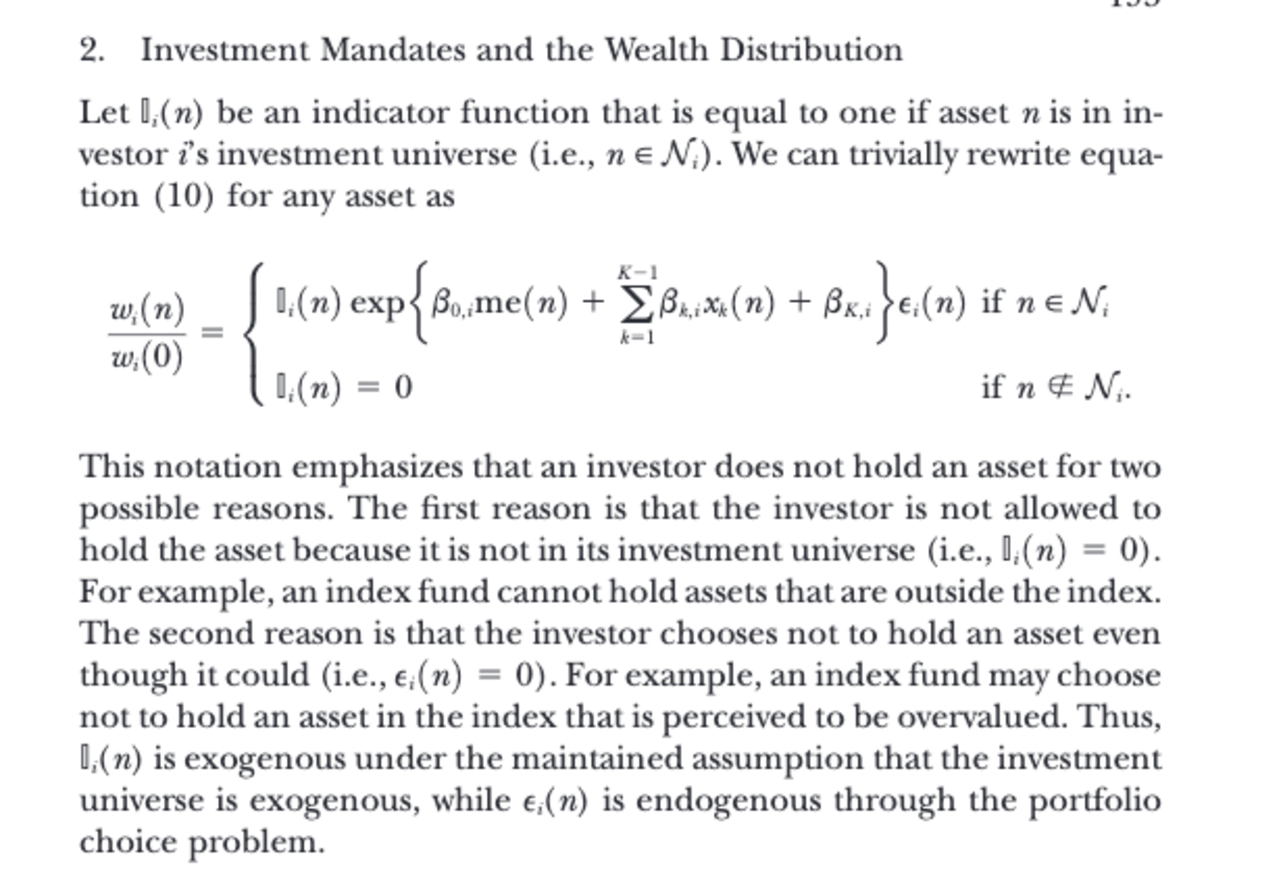
\includegraphics[width=\linewidth]{images/koijenyogo2.pdf}}                
  \end{column}
\end{columns}

\end{frame}

\end{document}
